%% To submit your paper:
\documentclass[draft]{agujournal2019}
\usepackage{lmodern}
\usepackage{url} %this package should fix any errors with URLs in refs.
\usepackage{makecell}
\usepackage{booktabs}
\usepackage{lineno}
% \linenumbers
\usepackage{multirow}
\usepackage[colorinlistoftodos]{todonotes}
\usepackage{pdfpages}
\usepackage{import}
% paragraph paragraph name (end)
% \draftfalse

\journalname{JGR: Solid Earth}
% As of 2018 we recommend use of the TrackChanges package to mark revisions.
% complete documentation is here: http://trackchanges.sourceforge.net

\begin{document}

%  TITLE
\title{Normal stress pulse during fluid-driven seismicity migration}

%  AUTHORS AND AFFILIATIONS
\authors{K. Ahmadov\affil{1}, J. Schmittbuhl\affil{1}, T.G.G Candela\affil{2}}
\affiliation{1}{EOST/ITES, Strasbourg University/CNRS, 5 rue René Descartes, 67000 Strasbourg, France}
\affiliation{2}{Geological Survey of the Netherlands, TNO, Utrecht, the Netherlands}
\correspondingauthor{}{}

% KEY POINTS
\begin{keypoints}
	\item
	\item
	\item
\end{keypoints}

%  ABSTRACT
\begin{abstract}
	Fractures play a significant role in fluid transport in a number of georesource applications. Here we study the fluid-driven reopening of a pre-existing fracture when the deformation along the fracture is significant, which has important implications for the initiation and migration of induced seismicity. We compare semi-analytical calculations of the pressure propagation in an elastically deformable fracture during fluid injection with numerical simulations using the Distinct Element Method (DEM) implemented in the 3DEC code (ITASCA).

	We show that the normal stiffness of the fracture is a key parameter. Soft fractures produce a sharp pressure front with a significant aperture change, whereas rigid fractures show a smooth and diffusive aperture and pressure distribution. In soft fractures, the sharp aperture/pressure front produces a pulse in normal tensile stress ahead of the propagating front. The amplitude of this stress pulse depends on the parameters of the problem, which we have analyzed through a sensitivity analysis.

	The propagation of the normal stress pulse follows a nonlinear diffusion equation in soft fractures, in contrast to the linear diffusion observed in rigid fractures. As a result, propagation is slower in fractures with lower normal stiffness, hence the fluid pressure migrates faster in the rigid fracture case. Despite these differences, the aperture and pressure fronts scale with $\sqrt{t}$ in both cases during constant-pressure injection.  In contrast, constant-rate injection produces migration with time exponents greater than 1/2. Increasing the injection rate further raises the exponent, approaching quasi-linear propagation with a constant front velocity.

	These results provide a mechanical explanation for the non-diffusive migration patterns observed at several fluid-injection sites and highlight the critical role of fracture deformability and injection protocol in controlling induced seismicity migration.

\end{abstract}

\section*{Plain Language Summary}

\section*{Conflict of Interest}
The authors declare no conflicts of interest relevant to this study.

%%%%%%%%%%%%%%%%%%%%%%%%%%%%%%%%%%%%%%%%%
%
%  BODY TEXT
%
%%%%%%%%%%%%%%%%%%%%%%%%%%%%%%%%%%%%%%%%%

\section{Introduction}

Seismic swarms are sequences of earthquakes that cluster in time and space. Unlike main shock-aftershock sequences, swarms lack distinct large earthquakes at the beginning of the sequence. Swarms occur naturally in diverse tectonic settings or can be induced by humans during industrial activities involving fluid injection or extraction from the subsurface \cite{ChenEtAl2012, DanreEtAl2024a}. A key feature in both natural and human-induced swarms is the migration of seismicity. Indeed, during most seismic swarms, the hypocenters migrate away from the initial events over time \cite{ShapiroEtAl2002, ChenEtAl2012, DeBarrosEtAl2021, DanreEtAl2024}. The spatial-temporal migration of swarm earthquakes is commonly analyzed in distance-time plots, where the distance of each event from the origin is plotted against the elapsed time. An important feature that often emerges from these plots is the seismic front, generally defined as the outer envelope of seismicity \cite{GoebelBrodsky2018, DanreEtAl2024}. Its evolution is often described by a power-law relationship in time:
\begin{equation}\label{eq:power-law-front}
	d(t) \propto t^{\alpha}
\end{equation}
where $d(t)$ is the distance from the origin at time $t$, and $\alpha$ is the exponent of time.

The existing literature on seismicity migration during swarms is extensive, with many studies focusing particularly on the time exponent $\alpha$ from Eq.~\ref{eq:power-law-front}. This parameter is of particular interest because its estimated value provides insight into the physical mechanisms driving seismicity \cite{ShapiroEtAl1997, ChenEtAl2012, GoebelBrodsky2018, DeBarrosEtAl2021, DanreEtAl2024}. Here, we briefly review reported values of $\alpha$ and the associated triggering mechanisms. Our discussion is limited to anthropogenic swarms, as natural swarms introduce additional uncertainties related to their greater focal depths \todo{provide a source}.
\subsection{Reported time exponents $\alpha$}

Early studies that identified and analyzed the power-law scaling in seismic front migration during earthquake swarms described its migration with a square root of time scaling ($\alpha=1/2$) \cite{ShapiroEtAl1997, ShapiroEtAl2002}.
Square root of time is a classical scaling of seismic migration with time and is observed at many injection sites \cite{GoebelBrodsky2018}.
In recent years there has been an increasing amount of research that showed that a different time exponent $\alpha$ explains the seismic front evolution at some injection sites.
The microseismicity induced during fluid injection operations at Barnett Shale and Cooper (in 2003) migrates close to cubic root of time $\alpha = 1 /3$ \cite{ShapiroDinske2009, JohannEtAl2016}.
Lately, studies found that fluid injection induced seismicity may also migrate with constant velocity ($\alpha=1$) \cite{LenglineEtAl2017, GoebelBrodsky2018, DanreEtAl2024}.
There are even cases where $\alpha$ increases with time. \cite{DeBarrosEtAl2021} showed that, at multiple sites, the first half of the sequence migrates with square root time and the second half has a linear migration pattern.
It is also important not to ignore the cases where seismicity lacks apparent migration behavior \cite{DuboeufEtAl2017, GoebelBrodsky2018}.
Table~\ref{tab:migration-observations} summarizes exponents of time $\alpha$ for seismic front migration reported for injection sites from the above mentioned sources. We can summarize the migration patterns into four general groups: square root of time, sub-1/2 exponents, quasi-linear or linear migration, and the lack of observable migration ($\alpha=0$). Interestingly, the reported $\alpha$ varies not only across different injection sites but also among different studies of the same site. This is evident in the case of Soultz 1993 and Basel injection experiments (Table~\ref{tab:migration-observations}). In conclusion, the literature of the analysis on seismicity migration data suggests that the seismic front evolution does not follow a single relationship in time, instead it changes with different injection sites and even among different researchers for the same site.

\begin{table}[htbp]
	\centering
	\caption{The exponent of time that describes the seismic front evolution given by the analysis of the dataset of anthropogenic seismic swarms various injection sites, as reported by different studies.}\label{tab:migration-observations}
	\begin{tabular}{llc}
		\toprule
		Site                              & Source                   & Time exponent, $\alpha$ \\
		\midrule
		\multirow{5}{*}{Soultz 1993}      & \cite{ShapiroEtAl2002}   & 1/2                     \\
		                                  & \cite{GoebelBrodsky2018} & 1/2                     \\
		                                  & \cite{DeBarrosEtAl2021}  & 0.65                    \\
		                                  & \cite{SaezUribe2023}     & 1                       \\
		                                  & \cite{DanreEtAl2024}     & 1                       \\
		\midrule
		\multirow{4}{*}{Basel 2006}       & \cite{JohannEtAl2016}    & 0.49                    \\
		                                  & \cite{GoebelBrodsky2018} & 1                       \\
		                                  & \cite{DeBarrosEtAl2021}  & 0.7                     \\
		                                  & \cite{DanreEtAl2024}     & 1                       \\
		\midrule
		\multirow{2}{*}{Cooper 2003}      & \cite{GoebelBrodsky2018} & 1/2                     \\
		                                  & \cite{JohannEtAl2016}    & 0.28                    \\
		Cooper 2012                       & \cite{DeBarrosEtAl2021}  & 0.5                     \\
		\midrule
		\multirow{2}{*}{Fenton Hill 1983} & \cite{ShapiroEtAl2002}   & 1/2                     \\
		                                  & \cite{GoebelBrodsky2018} & 1/2                     \\
		\midrule
		Rittershoffen 2013                & \cite{LenglineEtAl2017}  & 1                       \\
		Rittershoffen 2016-2024           & \cite{LenglineEtAl2025}  & 1/2                     \\
		\midrule
		KTB 1997                          & \cite{ShapiroEtAl1997}   & 1/2                     \\
		Barnett Shale                     & \cite{ShapiroDinske2009} & 1/3                     \\
		LSBB, France                      & \cite{DuboeufEtAl2017}   & 0$^1$                   \\
		St. Gallen                        & \cite{GoebelBrodsky2018} & 1                       \\
		Paralana, Australia               & \cite{GoebelBrodsky2018} & 1                       \\
		Landau                            & \cite{GoebelBrodsky2018} & 0                       \\
		Paradox, Colorado                 & \cite{GoebelBrodsky2018} & 1                       \\
		\bottomrule
		\multicolumn{2}{l}{$^1$ Seismic front lacks temporal dependence.}
	\end{tabular}
\end{table}

The dissimilarity in the interpretation of time exponents $\alpha$ across different authors for a given injection site arises from several factors. First factor may be the differences in methodological choices used to analyze seismicity migration. For example, the choice of spatial origin is inherently subjective and varies across studies \cite{DeBarrosEtAl2021}.
Similarly, the definition of the seismicity front may differ, as some studies define it as the 85-95th percentile of the farthest events \cite{DanreEtAl2024}, whereas others define it as the farthest events \cite{JohannEtAl2016}.
Second, the approach used to infer the time exponent $\alpha$ varies among studies.
Some authors \cite{JohannEtAl2016, DeBarrosEtAl2021, GoebelBrodsky2018} estimate $\alpha$ by fitting a power-law function to the observed migration, whereas others \cite{ShapiroEtAl2002, LenglineEtAl2017, SaezUribe2023, DanreEtAl2024} infer the front evolution from physical models and show that these predictions also explain the seismicity migration.
Last but not least, uncertainties in earthquake locations and the background noise can further affect the analysis \todo{provide a source}.

\subsection{Proposed triggering mechanisms}

Researchers have proposed several mechanisms associated with fluid-induced seismicity which attempt to explain the different exponents of time obtained for various injection sites. In the following, we briefly review the previously proposed triggering mechanisms and the associated scaling exponents $\alpha$ (Table~\ref{tab:induced-seismicity-mechanisms}).

Since the 1960s, injection-induced seismicity has been attributed to an increase in fluid pressure and an associated reduction in effective stress on pre-stressed faults and fractures \cite{HealyEtAl1968}.
Early studies therefore linked seismicity migration to linear fluid pressure diffusion, which predicts that fluid pressure perturbations migrate away from the injection point proportionally to the square root of time $\alpha=1/2$ (Table~\ref{tab:induced-seismicity-mechanisms}).
Initial observations of seismicity migration confirmed a similar scaling with time at multiple injection sites (Table~\ref{tab:migration-observations}; \citeA{ShapiroEtAl1997, ShapiroEtAl2002}), indicating that the seismic front follows the fluid pressure front.
However, subsequent studies found that, at several sites, the seismicity migration is better explained by a time exponent different from $\alpha=1/2$ (Table~\ref{tab:migration-observations}), which cannot be predicted by linear fluid diffusion (Table~\ref{tab:induced-seismicity-mechanisms}). The discrepancy between the classical model and the observations motivated researchers to seek alternative models with additional mechanisms.
For example, \cite{ShapiroDinske2009} proposed a model where the diffusivity of the porous medium depends on pore pressure, leading to nonlinear diffusion of fluid. This model predicts a time exponent $\alpha = 1/3$ when the flow is spherically symmetric (3D) and the applied injection rate is constant (Table~\ref{tab:induced-seismicity-mechanisms}).
This finding is consistent with the observations from Barnett Shale hydraulic fracturing and Cooper EGS site, where the seismicity expands with a cubic root of time $\alpha=1/3$.
% TODO: mention that nonlinear diffusion may also predict \alpha=1/2

\begin{table}[htbp]
	\centering
	\caption{Triggering mechanisms for injection-induced seismicity reported in the literature with their associated exponents of time and the injection sites.}\label{tab:induced-seismicity-mechanisms}
	\begin{tabular}{lllc}
		\toprule
		Mechanisms                           & Source                        & Site           & $\alpha$             \\
		\midrule
		\multirow{2}{*}{Linear diffusion}    & \cite{ShapiroEtAl1997}        & KTB, Germany   & \multirow{2}{*}{1/2} \\
		                                     & \cite{ShapiroEtAl2002}        & Soultz, France                        \\
		\midrule
		\multirow{3}{*}{Nonlinear diffusion} & \cite{ShapiroDinske2009}      & Barnett shale  & 1/3                  \\
		                                     & \cite{HummelMller2009}        & Fenton Hill    & 1/2                  \\
		                                     & \cite{JohannEtAl2016}         & Multiple sites & 1/2--1/3             \\
		\midrule
		\multirow{4}{*}{Aseismic slip}       & \cite{BhattacharyaViesca2019} & LSBB, France   & 1/2                  \\
		                                     & \cite{DeBarrosEtAl2021}       & Multiple sites & 0.7--1               \\
		                                     & \cite{SaezUribe2023}          & Multiple sites & 1/2--1               \\
		                                     & \cite{DanreEtAl2024}          & Multiple sites & 1                    \\
		                                     & \cite{DuboeufEtAl2017}        & LSBB, France   & 0                    \\
		\midrule
		Poroelasticity                       & \cite{GoebelEtAl2017}         & Oklahoma, USA  & 0                    \\
		\midrule
		Coulomb stress transfer              & \cite{YeoEtAl2020}            & Pohang, Korea                         \\
		\bottomrule
	\end{tabular}
\end{table}

In light of numerous observations of aseismic slip during fluid injection, recent studies have explored its role in the migration of induced seismicity \cite{GuglielmiEtAl2015b, BhattacharyaViesca2019, DeBarrosEtAl2021}. One of the first comprehensive analyses of fluid-driven aseismic slip predicted a time exponent for seismic front propagation that is consistent with the classical linear diffusion model ($\alpha = 1/2$) \cite{BhattacharyaViesca2019}. Incorporating aseismic slip can only increase the apparent diffusivity of seismicity migration when the fault is initially near a critically stressed state. Similar studies but with slightly different methods and different injection conditions such as constant or linearly increasing flow rate rather than constant pressure, demonstrated that fluid induced aseismic slip front can lead to quasi-linear or linear seismicity migration patterns ($\alpha \approx 1$) \cite{DeBarrosEtAl2021, SaezUribe2023, DanreEtAl2024}. These results show that in a aseismic-slip-driven regime the dependence of rupture front on time changes under different injection conditions.

At several injection sites, the seismicity lacks an observable migration pattern (Table~\ref{tab:migration-observations}). \citeA{GoebelBrodsky2018} suggest that lack of migration may result from far-reaching poroelastic stress changes which trigger earthquakes beyond the pressurized zones leading to different clusters of seismicity \cite{GoebelEtAl2017}.

Overall, Table~\ref{tab:induced-seismicity-mechanisms} shows that the predicted exponent of time $\alpha$ may or may not change with different physical mechanism governing the migration of earthquakes during anthropogenic swarms. A particular value of $\alpha$ does not give a conclusion on the triggering mechanism because one value of $\alpha$ may be reproduced by different governing mechanisms. Moreover, a particular triggering mechanisms can reproduce a range of values of $\alpha$. For example, aseismic slip driven regime can result in $\alpha$ being equal between 1/2 and 1, and nonlinear diffusion can reproduce $\alpha$ of 1/2 and 1/3. The predicted $\alpha$ strongly depends on the applied injection rate for both cases.

\subsection{Objectives}

In view of this conclusion of strong dependence of predicted exponent of time on the loading conditions. This dependence of the predicted exponent on the loading condition is what we aim to explore for a deformable pre-existing fracture. Our specific objective is to study how the coupling between fracture opening and fluid pressure influence the time dependence of the pressure front migration and hence the seismicity migration. For this purpose, we are going to extend the semi-analytical solutions provided by \citeA{MurphyEtAl2004, AhmadovEtAlInPrep} (\textit{in case it gets published}), combined with the numerical simulations using the Distinct Element Method (DEM). This will enable us to analyze the effect of injection rate on the pressure front migration and its scaling with time.

% A similar work has been done by \citeA{MurphyEtAl2004} where they predict $\alpha=4/5$ for a deformable fracture.This results aligns with some of the observations of seismicity migration seen in the literature (Table~\ref{tab:migration-observations}.Despite this fact, researchers have not treated the implications of such mechanisms on seismicity migration. Therefore, this study set out to investigate the effect of pressure-dependent fracture opening on the fluid pressure migration.
\section{Methods}

\subsection{Semi-analytical solution for aperture front migration}

The governing equation for aperture propagation in a deformable, parallel-plate, one-dimensional fracture subjected to fluid injection is the nonlinear diffusion equation \cite{MurphyEtAl2004}
\begin{equation}
	\frac{k_n}{12 \mu} \frac{\partial}{\partial x}\left(w^3 \frac{\partial w}{\partial x}\right)
	= \frac{\partial w}{\partial t},
	\label{eq:aperture-n3}
\end{equation}
where $w(x,t)$ denotes the fracture aperture, $k_n$ is the fracture normal stiffness, $\mu$ is the fluid viscosity, $x$ is the distance from the injection point, and $t$ is time.

\citeA{MurphyEtAl2004} derived a similarity solution to Eq.~\ref{eq:aperture-n3} for a semi-infinite fracture subject to constant injection rate $q_0$, assuming zero initial aperture. Under these assumptions, the problem admits self-similarity. That is, there exist dimensionless variables that transform Eq.~\ref{eq:aperture-n3} to an ordinary differential equation (ODE). The similarity variables are
\begin{equation}
	\theta(\zeta) = \frac{w(x,t)}{(q_0^2 t / a)^{1/5}},
	\qquad
	\zeta = \frac{x}{(a q_0^3 t^4)^{1/5}},
	\label{eq:dimensionless-variables-n3}
\end{equation}
where $\theta$ is the dimensionless aperture, $\zeta$ is the similarity coordinate, and
\[
	a = \frac{k_n}{12\mu}.
\]

If the aperture gradient is small such that $\left(\partial w / \partial x\right)^2 \approx 0$, Eq.~\ref{eq:aperture-n3} reduces to a linear diffusion equation. In this regime, the appropriate similarity variables become
\begin{equation}
	\theta(\zeta) =
	\frac{w(x,t)-w_i}{\left(q_0^2 t / (a w_i^3)\right)^{1/2}},
	\qquad
	\zeta = \frac{x}{(a w_i^3 t)^{1/2}},
	\label{eq:dimensionless-variables-n0}
\end{equation}
where $w_i$ denotes the initial aperture.

The fluid injection model under conditions described above is a limiting case for which a self-similarity exists \cite{Barenblatt1996}. One of these conditions is that the fracture has zero initial aperture prior to injection. If $w_i \neq 0$, strict self-similarity is lost because the far-field boundary condition becomes time-dependent. For a semi-infinite fracture, the initial aperture condition introduces another time-dependent dimensionless parameter
\begin{equation}
	\theta_{\infty} = \frac{w_i}{(q_0^2 t / a)^{1/5}}.
	% \label{eq:initial-aperture-boundary-condition}
\end{equation}
The parameter $\theta_{\infty}$ is a boundary condition that must be satisfied as $\zeta \to \infty$, hence the subscript $\infty$. When $w_i = 0$, the far-field condition is identically zero and independent of time, preserving self-similarity. In contrast, if $w_i \neq 0$, the boundary condition varies with time and the problem is no longer strictly self-similar.

Approximate self-similar solutions can be recovered in the early- and late-time limits. For this purpose, we define the critical (characteristic) time to be
\begin{equation}
	t_c = \frac{a w_i^5}{q_0^2}.
	\label{eq:critical-time}
\end{equation}
Using Eq.~\ref{eq:critical-time}, the far-field condition becomes
\begin{equation}
	\theta_{\infty} = \left( \frac{t_c}{t} \right)^{1/5}.
	\label{eq:critical-time-boundary-condition}
\end{equation}

When $t \gg t_c$, the aperture near the injection point greatly exceeds the far-field aperture. The influence of the initial aperture becomes negligible and the boundary condition effectively approaches zero. The problem asymptotically recovers the self-similar solution of nonlinear diffusion defined by the similarity variables in Eq.~\ref{eq:dimensionless-variables-n3}. In this regime, the aperture (or pressure) front position scales as
\begin{equation}
	d(t) \sim a^{1/5} q_0^{3/5} t^{4/5}.
	\label{eq:late-time-scaling}
\end{equation}

When $t \ll t_c$, the aperture remains close to its initial value and aperture gradients are small. The linear diffusion approximation applies (Eq.~\ref{eq:dimensionless-variables-n0}), yielding
\begin{equation}
	d(t) \sim (a w_i^3 t)^{1/2}.
	\label{eq:early-time-scaling}
\end{equation}

In summary, the fracture aperture (and equivalently pressure, due to their linear relationship) exhibits two asymptotic propagation regimes. At early times, $d(t) \propto t^{1/2},$ corresponding to diffusion-dominated behavior with exponent $\alpha = 1/2$. At late times, $d(t) \propto t^{4/5},$ corresponding to nonlinear aperture-controlled propagation with exponent $\alpha = 4/5$. For intermediate times $t \sim t_c$, the scaling exponent satisfies $1/2 < \alpha < 4/5,$ and increases monotonically from the diffusion-dominated limit toward the nonlinear asymptotic value.

\subsection{Numerical simulation}

We use a similar model setup as \citeA{AhmadovEtAlInPrep}. This model uses 3-D Distinct Element Code (3DEC, \citeA{Itasca3DEC2024}) to simulate fluid injection into a deformable pre-existing planar fracture. This model is hydromechanically fully coupled, in the way that fluid pressure, stress and hydraulic parameters of the model interact with each other during the numerical experiment.  The model is a 3-D model with dimensions of 100\,m\,×\,100\,m\,×\,100\,m (Figure~\ref{fig:model-schematic}). The horizontal fracture is contained in the middle of the elastic, homogeneous, isotropic, and impermeable rock block. We set the rock properties to typical values for a basement rock. We do not apply stress boundary conditions on the rock block, instead the block is under roller boundary condition on all edges except the right edge which is opposite to the injector. The fracture is not under initial stress and initial fluid pressure before the numerical experiment. We consider a fracture with a constant normal stiffness value that corresponds to large fractures ($k_{n}=50~\mathrm{GPa/m}$). The fracture has an initial aperture ($w_{i}$) of 0.1 mm (Figure~\ref{fig:model-schematic}). According to the cubic law \cite{WitherspoonEtAl1980}, the permeability corresponding to this initial aperture equals to $k=8.3 \times  10^{-10}~\mathrm{m^2}$. The properties of the fluid are same as of water. We inject the fluid along a line boundary at the onset of the fracture with a constant injection rate per fracture unit width. This simplifies the model into a 2-D problem with 1-D fluid flow. We analyze the effect of injection rate on the response of the model with multiple numerical experiment where we change the applied injection rate (Figure~\ref{fig:model-schematic}c).

\begin{figure}[htb!]
	\centering
	\import{figures_main/}{model-schematic.pdf_tex}
	\caption{(a) The sketch of the numerical model with an elastic rock block with roller boundaries on all edges except the right one, including a horizontal parallel-plate fracture in the middle. The fluid injection is applied at the inset of the fracture. The sketch draws the fluid overpressure induced relative opening of the fracture at the injection point during the simulation. (b) The drawing of the physical parameters of the fracture with a constant normal ($k_{n}$) and shear stiffness ($k_{s}$). The fracture has an initial aperture $w_{i}$. (c) Applied injection rate per simulation.}
	\label{fig:model-schematic}
\end{figure}

\newpage

\section{Results}

\begin{figure}
	\begin{center}
		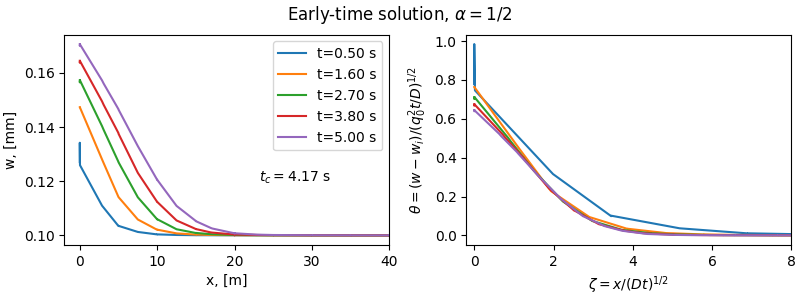
\includegraphics[width=0.95\textwidth]{figures_main/early-time-similarity.png}
	\end{center}
	\caption{Aperture profiles obtained at relatively early-times of the 3DEC simulation where applied injection flow rate equals $q_0=10^{-4}~\mathrm{m^2/s}$. (a) Dimensional aperture profiles obtained at multiple early-time steps (b) Dimensionless aperture profiles obtained using the self-similar variables (Eq.~\ref{eq:dimensionless-variables-n0}) approximated by early-time behavior}\label{fig:early-time-similarity}
\end{figure}

\begin{figure}
	\begin{center}
		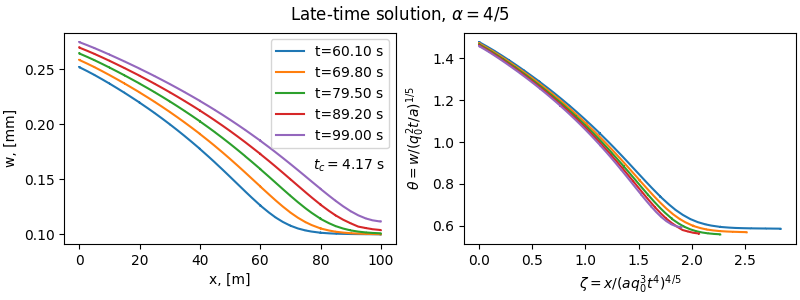
\includegraphics[width=0.95\textwidth]{figures_main/late-time-similarity.png}
	\end{center}
	\caption{Aperture profiles obtained at late-times ($t\gg t_c$) of the 3DEC simulation where applied injection flow rate equals $q_0=10^{-4}~\mathrm{m^2/s}$. (a) Dimensional aperture profiles obtained at multiple late-time steps (b) Dimensionless aperture profiles obtained using the self-similar variables (Eq.~\ref{eq:dimensionless-variables-n3}) approximated by late-time behavior}\label{fig:late-time-similarity}
\end{figure}

\begin{figure}
	\begin{center}
		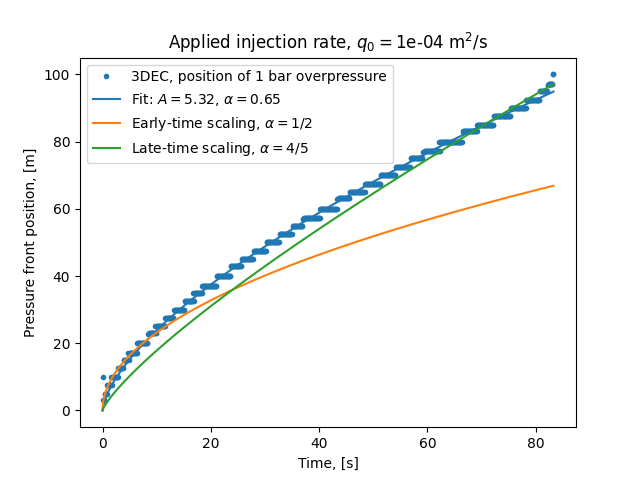
\includegraphics[width=0.95\textwidth]{figures_main/early-and-late-time-front-migration.png}
	\end{center}
	\caption{The migration of the position of 1 bar overpressure (pressure front) in time (blue dots) obtained from 3DEC simulation where applied injection flow rate equals $q_0=10^{-4}~\mathrm{m^2/s}$. Blue curve is the power-law fit to the front migration that gives best-fit prefactor of $A=5.32 $ and exponent of time $\alpha=0.65$. The orange curve is the front migration scaling in time obtained from the early-time approximation (Eq.~\ref{eq:early-time-scaling}) and the green curve is obtained from the late-time approximation (Eq.~\ref{eq:late-time-scaling})}\label{fig:pressure-front-migration}
\end{figure}

\begin{figure}[htbp]
	\begin{center}
		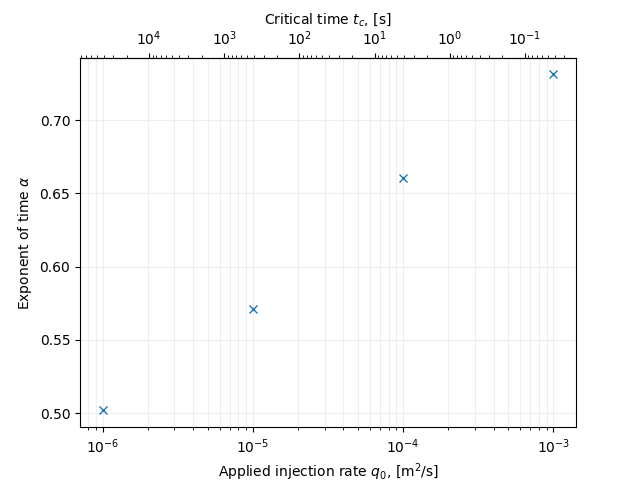
\includegraphics[width=0.95\textwidth]{figures_main/alpha_vs_q0.png}
	\end{center}
	\caption{Exponent of time $\alpha$ for front migration increases with applied injection flow rate. Critical time $t_c$ (Eq~\ref{eq:critical-time}) decreases with applied injection flow rate.}\label{fig:alpha-vs-q0}
\end{figure}

\begin{figure}
	\begin{center}
		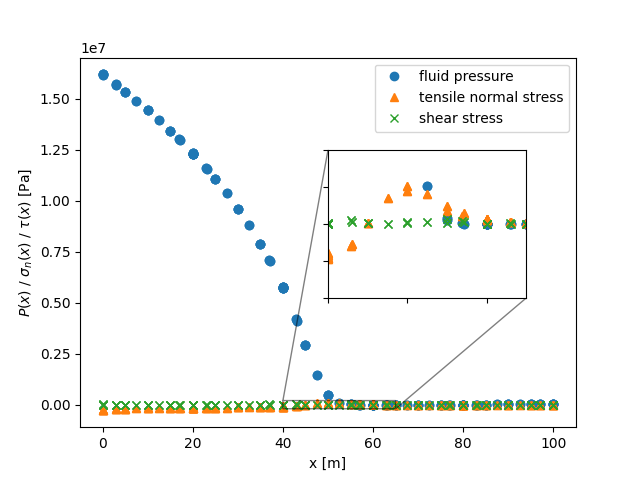
\includegraphics[width=0.95\textwidth]{figures_main/pressure-normal-shear-stresses.png}
	\end{center}
	\caption{Fluid pressure, tensile normal stress and shear stress along the fracture at $t=10~\mathrm{s}$}\label{fig:pressure-stress-profiles}
\end{figure}

\begin{figure}
	\begin{center}
		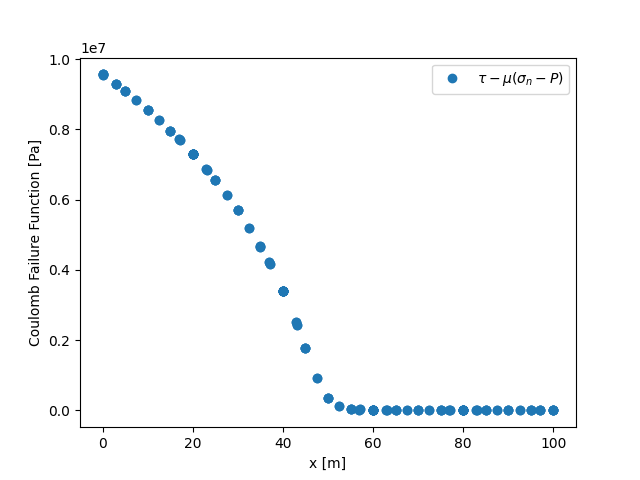
\includegraphics[width=0.95\textwidth]{figures_main/CFF.png}
	\end{center}
	\caption{Coulomb Failure Function ($\mathrm{CFF}= \tau(x) - \mu (\sigma_n(x) - P(x))$) along the fracture at time $t=10~\mathrm{s}$}\label{fig:CFF}
\end{figure}

\begin{figure}
	\begin{center}
		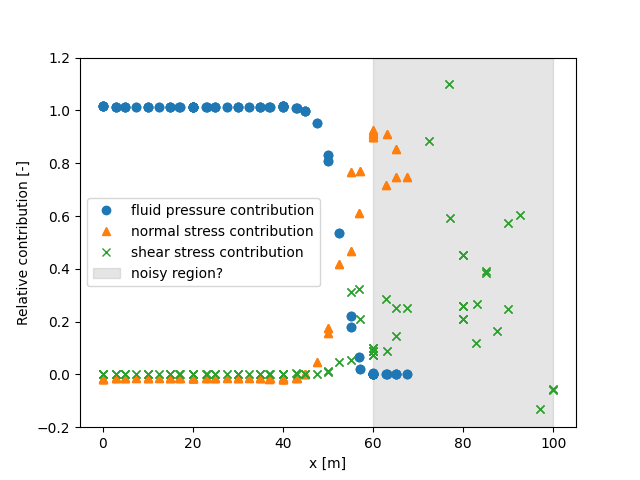
\includegraphics[width=0.95\textwidth]{figures_main/contribution-analysis.png}
	\end{center}
	\caption{Relative contribution of fluid pressure ($\frac{\mu P(x)}{\mathrm{CFF}(x)}$), normal stress ($\frac{-\mu \sigma_n(x)}{\mathrm{CFF}(x)}$), and shear stress ($\frac{\tau(x)}{\mathrm{CFF}(x)}$) to the Coulomb stress change}\label{fig:contribution-analysis}
\end{figure}

% \begin{figure}[htbp]
% 	\begin{center}
% 		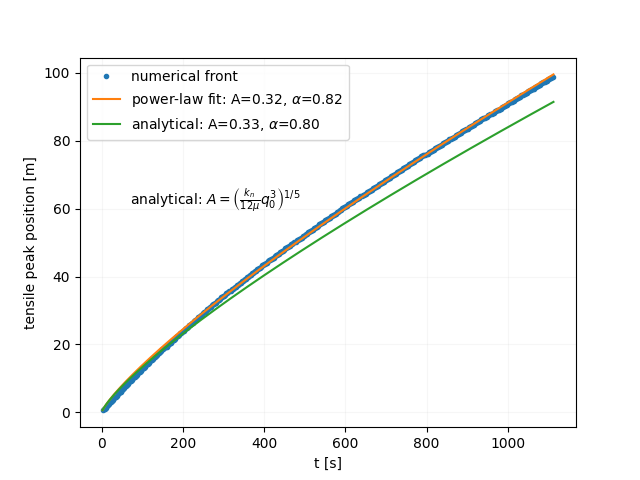
\includegraphics[width=0.95\textwidth]{figures_main/comparison-scaling-numerical-analytical.png}
% 	\end{center}
% 	\caption{Tensile stress peak distance in function of time obtained from numerical FVM simulation. The best fit power law exponent is $\alpha=0.82$ and a prefactor of $A=0.32$. A similarity scaling for initially impermeable fracture from \citeA{MurphyEtAl2004} predicts exponent of $\alpha=0.8$ with a prefactor determined by model parameters $A = \left( \frac{k_n q_0^3}{12 \mu} \right)^{1/5} = 0.33$ }\label{fig:comparison-with-analytical-scaling}
% \end{figure}
\newpage
%%%%%%%%%%%%%%%%%%%%%%%%%%%%%%%%%%%%%%%%%%%%%%%
%
% DATA SECTION and ACKNOWLEDGMENTS
%
%%%%%%%%%%%%%%%%%%%%%%%%%%%%%%%%%%%%%%%%%%%%%%%

\section*{Open Research Section}

\acknowledgments
This work of the Interdisciplinary Thematic Institut Geosciences for the energy system transition, as part of the ITI 2021-2028 program of the University of Strasbourg, CNRS and Inserm, was supported by Idex Unistra (ANR-10-IDEX-0002), and by SFRI-STRAT'US project (ANR-20-SFRI-0012).

\bibliography{references}

\end{document}
